    \vspace{-7pt}
\section{Introduction}\label{sec:intro}
    \vspace{-5pt}
% \begin{wrapfigure}[12]{r}{0.5\columnwidth}
%     \vspace{-12pt}
%     \centering
%     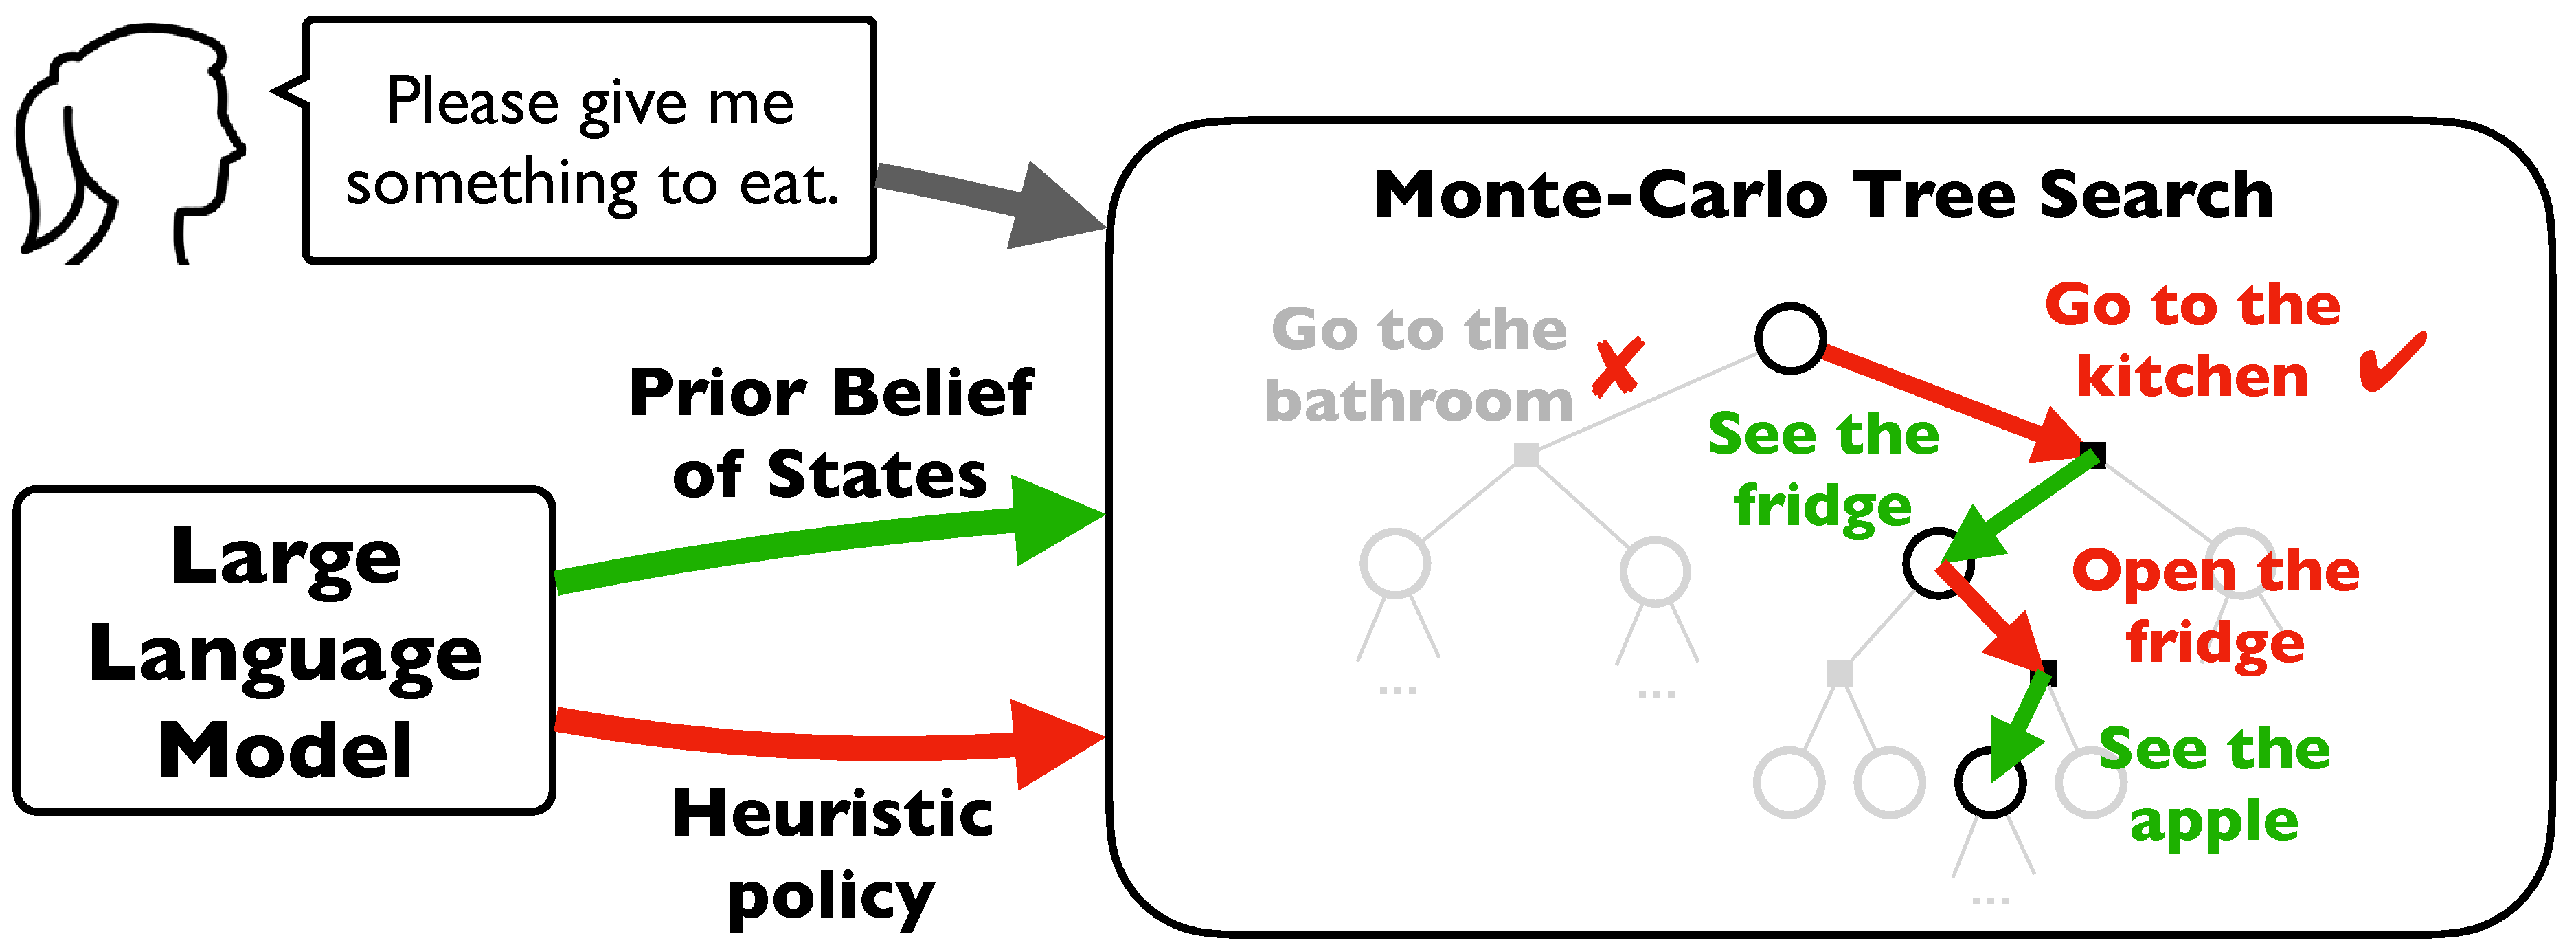
\includegraphics[width=0.5\columnwidth]{img/intro.pdf}
%     \vspace{-10pt}
%     \caption{We use the large language models as commonsense belief of states and heuristic policy to guide the Monte Carlo Tree Search to explore promising subtrees and make informed decisions.}
%     \label{fig:demo}
% \end{wrapfigure} 

%% object rearrangement task
Consider, for example, an autonomous robot butler in a household
environment. The human user sits in the living room and asks the robot to
"Put fruits into the fridge." The robot looks for fruits, such as apples,
peaches, \etc, which may be on a table in the dining room, on the kitchen
counter, but unlikely in a wardrobe in the bedroom. To complete the task, the
robot has to consider fruits' likely locations as well as their spatial
relations, traverse these locations efficiently, and finally put them into the
fridge.
A household environment typically contains hundreds of movable items and locations, resulting in a huge search space that makes the task very challenging for the robot.

%% L-Policy and L-Model
Recently, multiple attempts exploiting pre-trained large language models (LLMs) show surprisingly interesting results for such tasks \cite{li2022pre,huang2022language, ahn2022can, huang2022inner, brohan2022rt, zitkovich2023rt}. Their underlying idea is simple: treat the LLM as a policy and query it directly for the next actions, given the history of past actions and observations. We call this strategy \emph{L-Policy}, which exploits LLMs' vast commonsense knowledge to circumvent the challenge of searching a very large space. In our example task, L-Policy may simply instruct the robot to move to the hallway and then to the kitchen. 
% L-Policy works well if the induced policy is suitable for the task.
Even though LLMs are trained on internet-scale data, this strategy shows
limits in generalization \cite{dziri2023faith, berglund2023reversal},
especially when encountering uncommon, complex tasks. Alternatively, we may
use LLMs' knowledge to build a world model and apply a planning algorithm to
the model. The world model may contain, \eg,  a belief over  the
target object's location,
% For example, the fridge is usually in the kitchen even if the kitchen is not explicitly mentioned.
which biases the search and drastically improves search efficiency. We call
this strategy \emph{L-Model}. L-Model's performance depends on two critical
preconditions: the accuracy of the world model and the efficiency of the
planning algorithm. The former is a question of sample complexity for
learning, and the latter is that of computational complexity.

% classical model-based techniques \cite{kocsis2006bandit, coulom2007efficient,
%   browne2012survey, somani2013despot} employ random tree search sampling for
% large-scale problems but falter in vast domains due to sampling
% demands. Securing a robust model for these approaches is also pivotal. To
% address these challenges, several studies \cite{silver2017mastering,
%   silver2018general, cai2019lets, schrittwieser2020mastering} integrate
% learning with model-based planning to reduce the search space and learn a
% model, albeit at the expense of significant data needs. An intriguing question
% is: Can we use LLMs directly as a model in model-based algorithms to achieve
% more effective planning?


%% LLM-MCTS
This paper presents LLM-MCTS (shown in Fig \ref{fig:overview}), which combines the ideas of L-Model and L-Policy
for large-scale task planning. Like L-Model, LLM-MCTS uses an LLM to build a commonsense world model; it then uses the model to perform Monte Carlo Tree Search (MCTS)~\cite{coulom2007efficient} online for the next actions. During the tree search, LLM-MCTS chooses the promising action branches heuristically by querying the LLM. This is similar in spirit to L-Policy. While L-Policy commits to the actions chosen by the LLM for execution, LLM-MCTS uses these choices only as a search heuristic.

We evaluate LLM-MCTS in VirtualHome \cite{puig2018virtualhome}, a standard
household activity simulation platform, widely used in earlier
work~\cite{huang2022language, li2022pre, puig2020watch, Singh2023progprompt}. 
The evaluation set consists of 800 randomly generated large-scale, partially observable object rearrangement tasks, which aim to place common household objects in designated locations. Our main experimental findings are summarized below:
\begin{itemize}
\item[F1.] \emph{L-Model performs poorly.}  There are two possible
  reasons. One is model inaccuracy. The other is huge search space size,
  beyond the reach of even the state-of-the-art MCTS algorithm. Further
  experiments indicate that search space size is the main cause.
\item[ F2.] \emph{L-Policy performs reasonably with both GPT2 and GPT3.5, but the performance degrades quickly for novel, complex tasks.} This generally corroborates with earlier results~\cite{li2022pre,huang2022language, ahn2022can, huang2022inner}.
\item[F3.] \emph{LLM-MCTS outperforms L-Model.} This clearly shows the benefit of using the LLM as a heuristic policy to guide the search.
\item[F4.] \emph{LLM-MCTS outperforms L-Policy, especially for novel, complex
    tasks.}  LLM-MCTS basically combines L-Model and L-Policy. Since the
  L-Model performs very poorly on its own, why does the combination outperform
  L-Policy? One explanation is that search space size is the main cause of
  L-Model's poor performance. The LLM-induced world model is sufficiently
  accurate, and tree search with this world model, when limited to the neighbourhood of the LLM-induced policy, provides the improved performance over L-Policy. 
\end{itemize}



The explanation for (F4) begs a new question: with an efficient planning
algorithm for large search space, \emph{would L-Model outperform L-Policy?} To
answer this question, we study two related, simpler tasks: multiplication of
two large numbers and multi-hop travel planning. We discuss
multiplication here and travel planning in \secref{sec:air-plan}. A decimal
number is described as a sequence of $n$ digits,
$(d_{n-1}, d_{n-2}, \dots, d_0)$. There are two methods of implementing
multiplication with an LLM. The first one corresponds to L-Policy. We
represent the multiplication function as a table. Each row or column
corresponds to a number. The table entry is the multiplication of two numbers,
obtained by querying an LLM. Experimentally, GPT4 performs single-digit
multiplication perfectly with $100\%$ accuracy, 2-digit multiplication with
$99\%$ accuracy, 4-digit multiplication with merely $4\%$ accuracy, and fails
almost completely on 5-digit multiplication~\cite{dziri2023faith}. The second approach uses LLM-derived small single-digit multiplication tables, which GPT4 performs with 100\% accuracy. To multiply multi-digit
numbers, it applies the long multiplication algorithm with the single-digit
table. This method corresponds to L-Model. While long multiplication 
differs from planning in algorithmic details, it plays the same role in L-Model and is highly
efficient. Clearly, this second method achieves $100\%$ accuracy for arbitrarily
large numbers, provided that the single-digit multiplication table is
accurate. So, the L-Model outperforms L-Policy for the multiplication
task, contrary to the finding for object rearrangement tasks.

\emph{How do we choose between L-Model and L-Policy then? } One idea is the
minimum description length (MDL) principle. Theoretical analysis suggests that
a hypothesis with a shorter description length has a smaller generalization
error and is preferred~\cite{shalev2014understanding}. For multiplication, the
method corresponding to L-Policy uses a large table of $O(10^{2n})$
entries. It takes $O(n 10^{2n})$ bits to represent it. The method
corresponding to the L-Model uses a single-digit multiplication table of
constant size. The long multiplication algorithm can be encoded in any
reasonable programming language with constant size. So, the total
representation size is constant. According to MDL, the L-Model has a smaller
generalization error than the L-Policy for multiplication, with sufficiently
large $n$. This is fully consistent with experimental
results~\cite{dziri2023faith}. The analysis of travel planning
provides further evidence (\secref{sec:air-plan}).

In summary,  LLM-MCTS combines the ideas of L-Model and L-Policy,
outperforming either alone for complex task planning, particularly, object
arrangement (Sections \ref{sec:llm-mcts} and \ref{sec:main_experiments}).  To
choose between L-Model and L-Policy, MDL provides a useful guiding principle
(Section \ref{sec:mdl}). In essence, simplicity is preferred, a well-known
general principle in machine learning.


% This study uses LLMs as both the commonsense world model and the
% heuristic policy within Monte Carlo Tree Search (MCTS)
% \cite{coulom2007efficient}. MCTS utilizes LLMs' rich world knowledge for
% reasoned decision-making, which is not fully exploited when LLMs are used
% solely as policies. Specifically, LLMs provide prior common sense beliefs of
% the world that can be used to sample likely states that encompass common
% scenarios, such as fruits being present on the kitchen counter, inside the
% fridge, or in the pantry. {The prior common sense belief effectively reduces
%   the belief space for search in a large domain.}
% % MCTS summarizes the useful
% % information in searching the likely states through the estimated $Q$ value
% % (the expected return after taking action) to make a reasonable decision. The
% % algorithm progressively updates its belief of the world as it acts in the
% % world and receives observations to rectify model errors.

% In addition, instead of directly providing instructions, we employ the LLM as a search heuristic to
% guide exploration only toward promising parts of the search tree. For
% instance, when given the instruction "bring me a fruit," the LLM uses
% commonsense knowledge to prioritize opening the fridge or pantry rather than
% opening the trash can. Using LLM policies as search heuristics, we transform
% an otherwise intractable search task into a computationally practical one.

%% LLM-MCTS experimental findings and interpretation
% In contrast to solely using LLMs as policies, our method is able to exploit knowledge about likely states of the world in the LLMs to facilitate reasoned planning through tree search.
% % \footnote{For the purpose of the search, we assume that the action set is known with known deterministic transitions. In the experiments, the physical-level motion planning is processed separately when executing an action.} 
% MCTS enables LLM to leverage its world modelling knowledge and explore new combinations of actions to tackle novel tasks. LLM's initial belief of states effectively reduces the belief space for search in a large domain. LLM heuristic policy substantially reduces the search complexity required to identify good actions. We demonstrate the advantages through our experiments conducted in large, complex household environments, specifically in the context of daily task planning.


% The question arises as to whether the knowledge of LLMs regarding states of the world is more complete than their knowledge of policies for accomplishing daily tasks.
% {
% \color{blue}
% To discern the efficacy of using LLM as a model, we use the \emph{Minimum Description Length (MDL) principle} to compare its use as a planning policy \emph{(L-Policy)} versus its general application in a model-based approach \emph{(L-Model)}. We discovered that for a certain real-world domain, if the description length of the world model is shorter than the policy, the L-Model is a better option than L-Policy. {\color{purple}Given a description language, the description length can be evaluated by the required bits of space complexity for describing an instance of the prediction rule. We take $n$-digit multiplication with a binary-encoded description language as an example. The policy prediction rule and the 1-digit multiplication rule can be represented by a 2-dimensional table, where each column and row denotes two input numbers for multiplication, and the table entry is the result.} Describing the policy, encompassing all multiplications of two $n$-digit numbers, necessitates approximately $O(n10^{2n})$ bits. Conversely, a model description, encompassing digits 0-9 and their multiplication demands roughly $O(10^{2})$ bits. According to MDL, the error rate of the L-Policy is higher than the L-Model, which is also shown in \cite{dziri2023faith}. However, the L-Model can manifest compounded errors due to imperfect LLM modelling. We demonstrate in the Appendix \ref{app-sec:multiplication} that for a significant description length discrepancy between the L-Model and L-Policy, a large $n'$ exists where, if $n<n'$, the L-Model is optimal. Otherwise, both methods should perform poorly if $n\geq n'$ or equally well when $n$ is very small.

% %% DL analysis
% The nature of multi-digit multiplication, characterized by multi-step reasoning and compositionality, aligns with the core feature of planning. To fortify our MDL-based conclusions in the realm of planning, we delved into air travel and household task planning analyses. Both analytical and empirical evidence underscores the MDL's applicability in utilizing LLM for task-planning problems. While our research primarily focuses on large-scale task planning, the implications might extend to multi-step reasoning problems broadly. Notably, a study \cite{dziri2023faith} also suggests that the transformer LLMs are inherently limited for compositional, multi-step reasoning. Thus, using the L-Model for general reasoning problems is a promising direction to explore.  
% }



% Given that LLMs can be used as both models of the world and policies for selecting actions, one question is whether an LLM's knowledge about the states of the world is more complete than its knowledge of policies to complete daily tasks. While this question can only be settled empirically for real-world problems, we argue that LLM models are likely to be more complete than the LLM policies for some real-world domains \footnote{Here, we describe a simple problem where learning about the world would likely require less training data than learning policies to do all tasks in the domain. Consider the task of planning for air travel from a starting city to a destination city. To be able to solve the problem through a planning process, we only need to know the direct flights out of each city. This can be modeled as a graph, which is likely to be sparse in the real world. Assuming that the total number of edges grows proportionally to the number of cities, $O(n\log n)$ bits would be sufficient to describe a graph with $n$ cities, with approximately $2\log n$ bits used to describe the two cities involved in each edge. On the other hand, considering all possible start and destination cities already give about $n^2$ tasks. If we assume that each task requires a constant number of flights, we need to specify about  $n^2$ trajectories, requiring the order of $n^2\log n$ bits. The amount of data required for learning to solve a problem typically depends on the complexity of a problem, which can roughly be estimated by the description length of the solution. In this example, the total description length of policies is far larger than the description length of the model.} and performing a search using LLMs for such problems may be more successful than using the LLMs as policies. At the very least, it is likely useful to exploit the LLM as both a model as well as a policy, which we do in our work.

% Specifically, we leverage the commonsense knowledge from large language models as heuristics for Monte Carlo Tree Search, and we apply the method to solve language-conditioned task planning problems in complex household environments. The commonsense policy prior encourages the agent to search for promising directions that might solve the problem. For example, to achieve "bring me an apple," we will intuitively follow the commonsense to open the fridge instead of switching off the light. On the other hand, when the items' positions are out of observation or contradict our memory, we will also have the commonsense knowledge to predict their position. For example, if the apple is not in the fridge, it might be on the kitchen shelf. Those heuristics will substantially benefit planning, especially for large, complex environments with rich searching space. 

%Our method substantially improves the planning correctness of large language models while maintaining their usefulness and efficiency w.r.t commonsense knowledge. 


% In contrast to previous works, which typically use LLMs to provide instructions conditioned on previous observations as a policy, we use the commonsense knowledge embedded in the LLMs as a model to sample likely states of the world in order to do the planning. We simultaneously use the LLM as a policy, not to provide instructions directly but to help guide the planning process. LLMs contain a lot of world knowledge that is not exploited when they are used only as policies, and we show that additionally exploiting knowledge about likely states of the world can improve performance substantially. 

% One natural question is whether the knowledge that LLMs have about the states of the world is more complete than the knowledge they have about policies to achieve tasks that we would like to do. While this question can only be settled empirically for real-world problems, we describe a simple problem where learning about the world would require less training data than learning to do all tasks in the domain. Consider the task of planning a trip from a start city to a destination city. To be able to solve the problem through a planning process, we only need to know the direct flights out of each city. This can be modeled as a graph, which is likely to be sparse in the real world. Assuming that the number of edges grows proportionally to the number of cities, $O(n\log n)$ bits would be sufficient to describe a graph with $n$ cities, with approximately $2\log n$ bits used to describe the two cities involved in each edge. On the other hand, considering all possible start and destination cities already give about $n^2$ tasks. If we assume that each task requires a constant number of flights, we need to specify about  $n^2$ trajectories, requiring of the order of $n^2\log n$ bits. The amount of data required for learning to solve a problem typically depends on the complexity of a problem, which can roughly be estimated by the description length of the solution. In this example, the total description length of policies is far larger than the description length of the model. In practice, given a fixed amount of data available to train an LLM, we argue that the LLM model is likely to be more complete than the LLM policy for some real-world domains. At the very least, it is likely useful to exploit the LLM as both a model as well as a policy, which we do in our work.



% Assume a house consists of various interactive items, including $n$ grabbable objects, $m$ containers, and $k$ rooms. The available actions are picking/placing grabbable objects, walking to an object or a room, or opening/closing a container. Therefore, the size of the action space is roughly proportional to the number of objects $|A|\propto (n+m+k)$. As natural language uses object-centric relations to describe a state, such as "apple is on the table" and "fridge is in the kitchen." Therefore, the state can be represented as a sparse graph, requiring $O(n\log(m+n) + m\log(m+k))$ bit to describe. We assume a task is specified by a pair of objects (e.g., "put an apple inside a fridge" is paired with an "apple" and a "fridge."). A solution to finish a task is specified by several objects connected by actions, represented as a path in a graph (e.g., "grab the apple, walk to the kitchen, walk to the fridge, open the fridge, put the apple inside the fridge" is a path where the actions are its edges and objects are its nodes). Therefore, specifying a primary task requires $O(n^2)$ bits, resulting in $O(mn\log(m+n+k))$ to describe all the solutions. When composing multiple tasks, the description complexity further grows to $O((mn)^N\log (m+n+k))$, where $N$ is the number of composed tasks. Therefore, describing a policy is more complex than a model.




%%% Local Variables:
%%% TeX-master: "./main"
%%% End:
